\documentclass[11pt]{article}

\usepackage{mathpazo}
\usepackage{upgreek}
\usepackage{fullpage}
\usepackage{graphicx}
\usepackage{booktabs}                      % beautiful tables
\usepackage{caption}                       % allow multi-line captions
\usepackage{afterpage}
\usepackage{tabularx}
\usepackage{enumitem}
\usepackage{longtable}
\usepackage{parskip}
\usepackage{multirow}

\setlength{\parskip}{\baselineskip}
\setlength{\parindent}{0pt}

%% and here the glossaries package is... ------------------
% \usepackage{glossaries}
% \makeglossaries

% % regular acronym
% \newcommand{\acr}[1]{\gls{#1}}

% % plural acronym
% \newcommand{\acrpl}[1]{\glspl{#1}}

% % short version acronym (for captions, titles, etc)
% \newcommand{\acrsh}[1]{\glsentryshort{#1}}

% % short and plural acronym (for captions, titles, etc)
% \newcommand{\acrshpl}[1]{\glsentryshortpl{#1}}

% % creates acronym and also helper commands to ease use during writing
% \newcommand\makeacronym[4][]{
%   \newacronym[#1]{#2}{#3}{#4}
%   \expandafter\newcommand\csname #2\endcsname[1][]{%
%     \csname acr##1\endcsname{#2}\xspace%
%   }
% }

%% to make a ref for table and figures. Notice label prefix, which
%% means you should include those in the labels when including the
%% figure, but you don't need to put them when using the commands
%% below. This guaranties that you are not misplacing a figure in the
%% place of a table, or the other way around.
\newcommand{\figref}[1]{Figure~\ref{fig:#1}}
\newcommand{\tabref}[1]{Table~\ref{tab:#1}}
\newcommand{\secref}[1]{Section~\ref{sec:#1}}

% links and glossaries

\usepackage{hyperref} % hyperlinks, always last but glossaries


\title{ETL Readout Board Design}
\author{Indara Suarez, Daniel Spitzbart, Andrew Peck, Eric Hazen, Shouxiang Wu
  \\
  \\ \Large{\textbf{Boston University}}}

\date{\today}

\begin{document}

\maketitle

\tableofcontents

\section{Introduction to the Flipped Module Design}

This document describes an alternative of the ETL module and service hybrid design to the TDR design.
In this proposal the LGAD silicon sensor is located below the read out chip (ETROC), essentially flipping the TDR module on its head.
A PCB can be mounted (glued) on top of the ETROC, allowing for a board-to-board connection to the readout board (RB).
Signals, LV and bias voltage (BV) are distributed from the RB to the module via these board-to-board and spring connectors.
The ETROC and the LGAD sensor are connected to the PCB through wire bonds.
The main motivation for this revised RB and module design are the tight space restrictions for the service hybrid in the TDR design, which are relaxed if the RB sits on top of the modules instead of on top of the power board in the service channel between the modules.

\begin{figure}[!h]
\centering
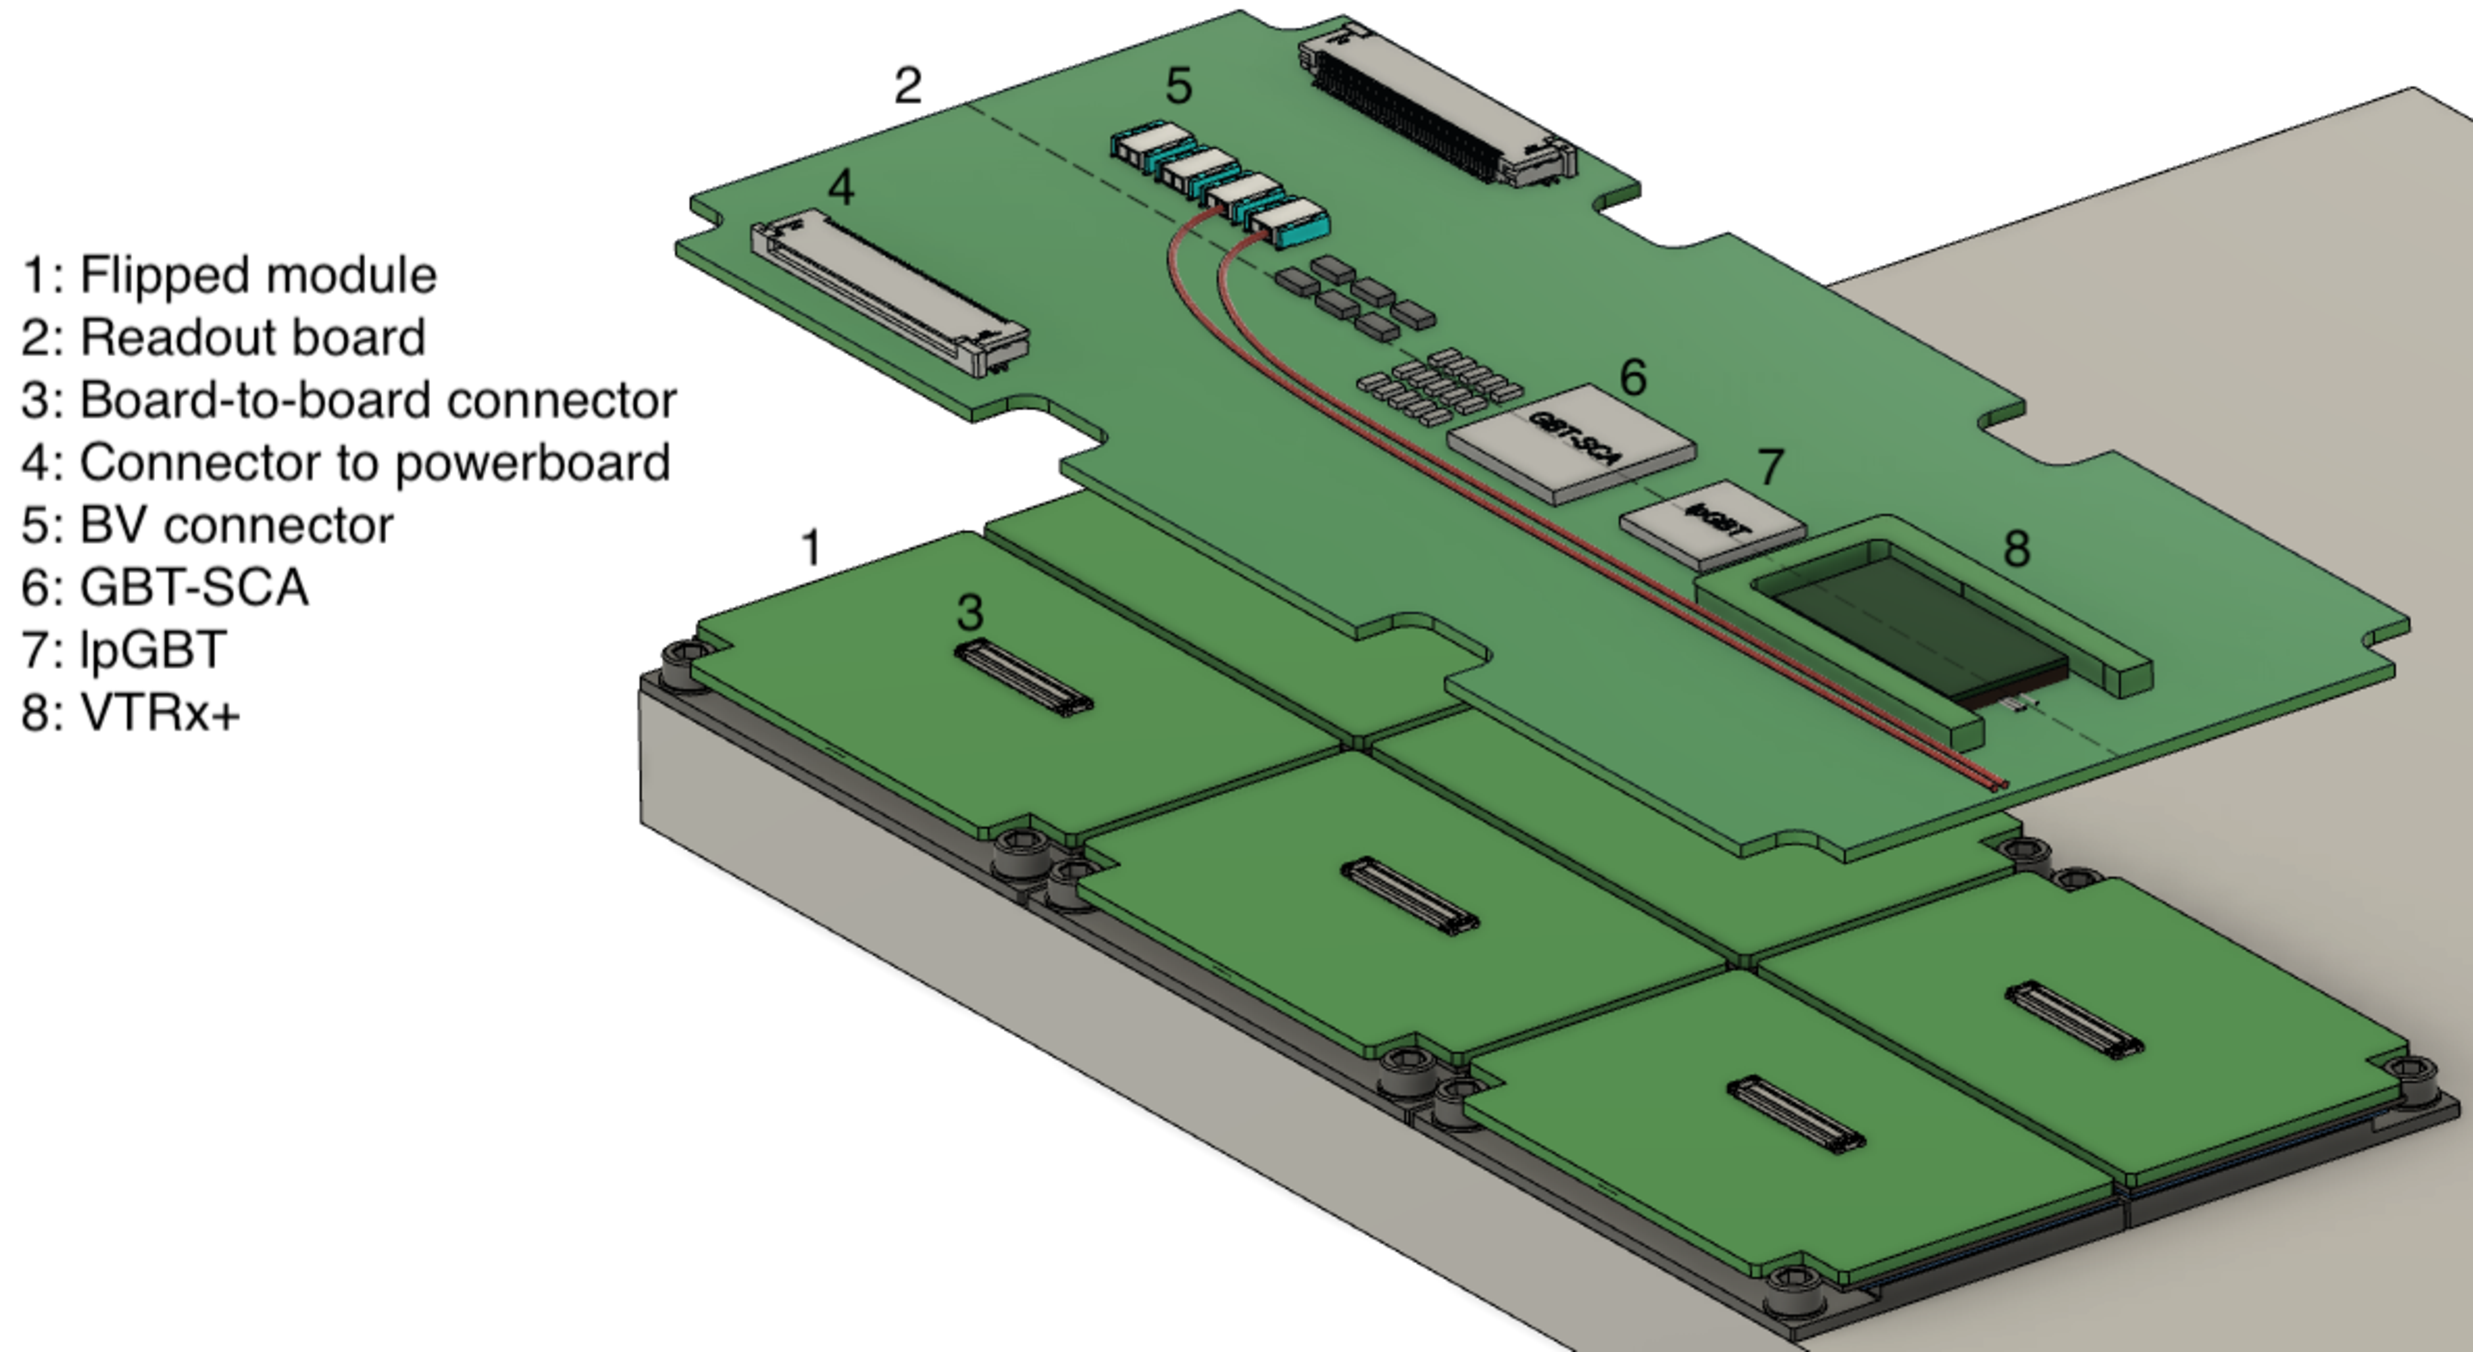
\includegraphics[width=0.90 \textwidth]{figures/ETL_exploded_legend.pdf}
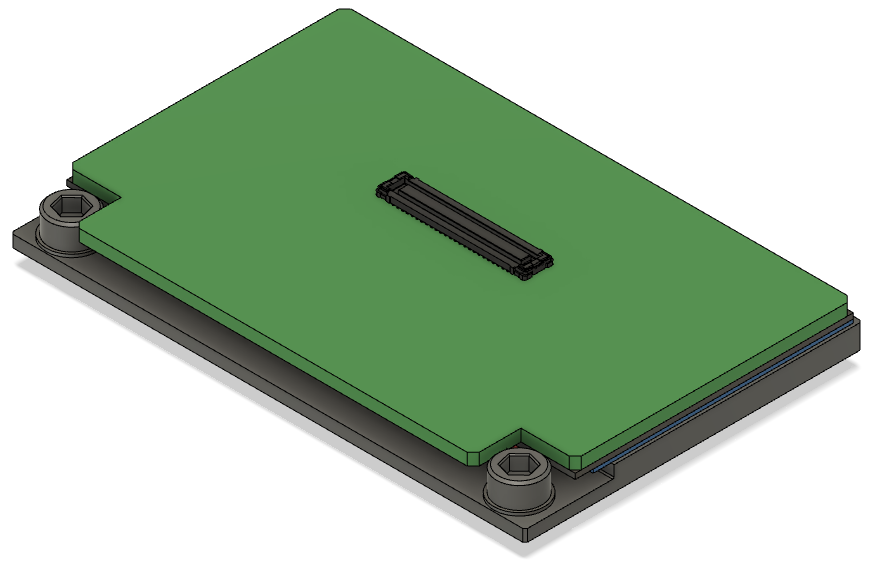
\includegraphics[width=0.40 \textwidth]{figures/Flipped_module_3D_v2.png}
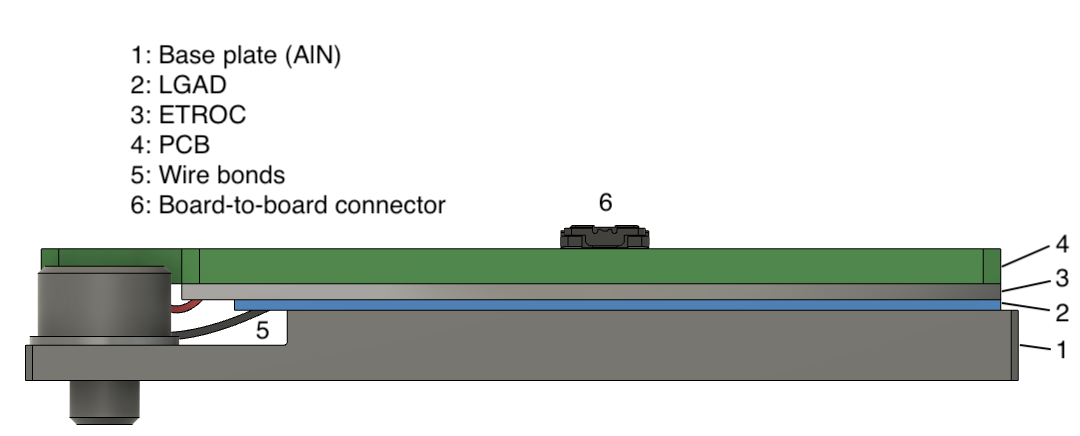
\includegraphics[width=0.55 \textwidth]{figures/Flipped_module_legend_v2.png}
\caption{
Top: Partially exploded views of the module-RB sandwich showing its various components.
Bottom: View of a half module in the flipped configuration, with the LGAD sensor below the ETROC.
}
\label{fig:flippedModule}
\end{figure}

We forsee three different versions of the RB: covering 3 (6), 6 (12) and 7 (14) full (half) modules.
Each full module consists of two LGAD sensors and four readout chips (ETROC).

The expected radiation environment for various regions are shown in Table 1.
To deal with higher occupancy in high-$|\eta|$ regions the innermost part of the ETL disk ($r<425~\mathrm{mm} \equiv |\eta|>2.65$) will be populated by 3-module readout boards.
The rest of the disk is organized such that the area coverage of the detector with sensors is optimized.
The layout of modules and service hybrids on the surface of the ETL wedges is presented in Figure~\ref{fig:coverage}.
Very good coverage between $1.7<|\eta|<2.8$ is achieved, without the need for half-sized modules.
We reserve an area of the width of RB and PB with a depth of 50 mm at the outer edge of the disks for MT connectors as well as LV and BV distribution, shown in Fig.~\ref{fig:patchpanel}.
The main difference w.r.t. the TDR design in terms of service hybrids is the placement of the RB on top of the modules, instead of the power board.
The RBs are powered either from above or below (powered from above shown in Fig.~\ref{fig:coverage}).

\begin{figure}[!h]
\centering
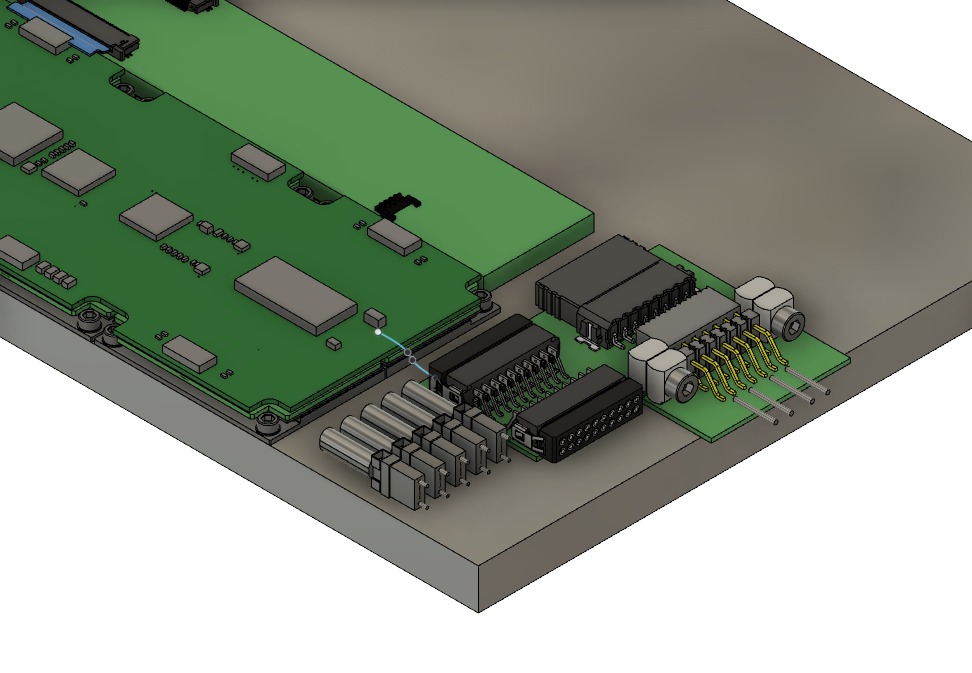
\includegraphics[width=0.70 \textwidth]{figures/patch_panel_3D.png}
\caption{
Mini-patch-panel at the end of each row of RBs and PBs.
}
\label{fig:patchpanel}
\end{figure}


\begin{table}
  \centering
  \caption{Table 1: Nominal radiation doses and fluences at various locations of the timing layers after 3000 fb$^{-1}$. The fluence is normalized to 1 MeV neutron equivalent in silicon.
  Numbers from [1]}
  \label{table:radiationField}
  \begin{tabular}{ c c c c c c }
    Region & $\eta$ & R (cm) & z (cm) & Fluence (cm$^{-2}$) & Dose (kGy) \\
    \midrule
    barrel & 0.0    & 116    & 0      & 1.65$\times 10^{14}$ & 18         \\
    barrel & 1.15   & 116    & 170    & 1.80$\times 10^{14}$ & 25         \\
    barrel & 1.45   & 116    & 240    & 1.90$\times 10^{14}$ & 32         \\
    endcap & 1.6    & 127    & 303    & 1.5$\times 10^{14}$ & 19         \\
    endcap & 2.0    & 84     & 303    & 3.0$\times 10^{14}$ & 50         \\
    endcap & 2.5    & 50     & 303    & 7.5$\times 10^{14}$ & 170        \\
    endcap & 3.0    & 31.5   & 303    & 1.6$\times 10^{15}$ & 450        \\
  \end{tabular}
\end{table}

\begin{figure}[!h]
\centering
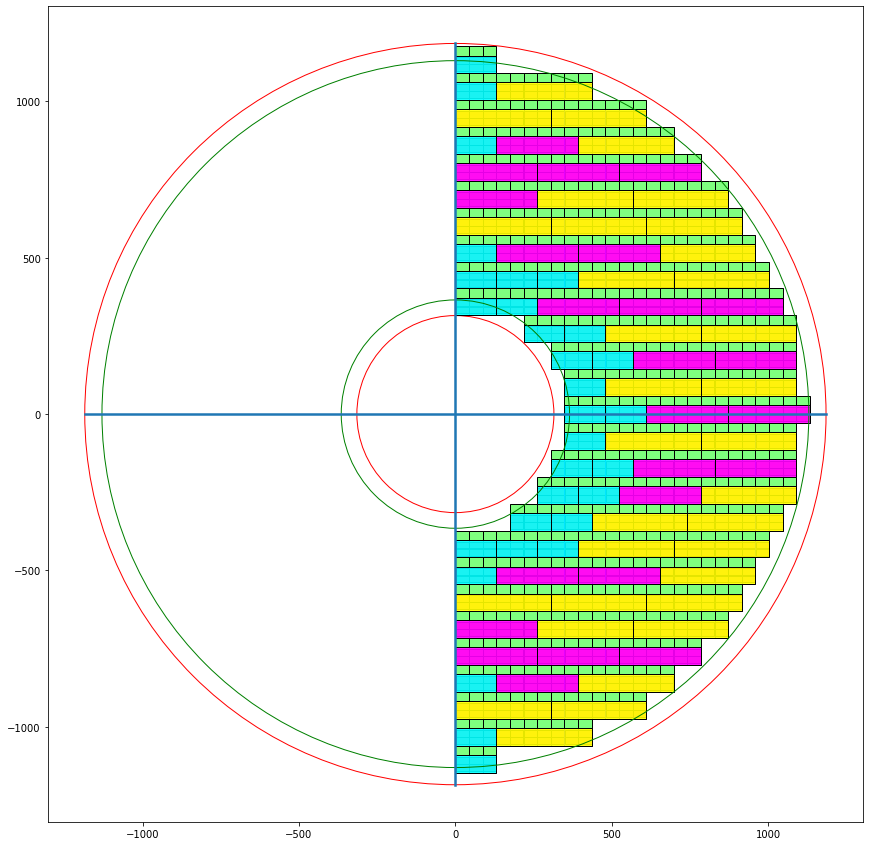
\includegraphics[width=\linewidth]{figures/coverage.png}
\caption{
Layout of various kinds of RBs on an ETL half-disk.
The red and green circles reflect the mechanical envelope of the ETL disk and the area between $1.7<|\eta|<2.8$, respectively.
Cyan, pink and yellow rectangles correspond to 3-, 6-, and 7-module readout boards.
The green rectangles indicate the reserved space above the RB for the power boards and LV services.
}
\label{fig:coverage}
\end{figure}

\begin{table}
  \caption{List of the number of each type of component used in the full ETL detector.}
  \centering
  \begin{tabular}{ l c c }
    Component type               & Number per wedge (avg) & Total number \\
    \midrule
    LGADs                        & 930             & 14,880      \\
    ETROCs                       & 1,860           & 29,760      \\
    2-sensor (full size) modules & 465             & 7,440       \\
    1-sensor (half size) modules & 0               & 0       \\
    total service hybrids     & 86.5               & 1,384       \\
    3-module service hybrids  & 28.5               & 456         \\
    6-module service hybrids  & 26.5               & 424         \\
    7-module service hybrids  & 31.5               & 504         \\
    lpGBTs, VTRX, SCA         & 86.5               & 1,384       \\
    DC-DC converters \textbf{need updated numbers!}          & \textit{893}    & \textit{14,288}        \\ %9 per full-size and 5 per half-size
  \end{tabular}
  \label{tab:ETLNumberOfComponents}
\end{table}

\section{Changes to the Module Design}

In this proposal, no half size modules are foreseen.
The modules itself have a changed structure, shown in Figure~\ref{fig:flippedModule}:
\begin{itemize}
  \item A thicker carrier (approx. 1 mm) made out of Aluminium nitride (AlN) or Aluminium oxide (alumina)
  \item The LGAD sensor is directly mounted to the carrier, below the ETROC
  \item The LGAD (BV) and ETROC (signals and LV) are wire bonded to a PCB that covers the module
  \item The module is connected to the readout board via board-to-board connectors
\end{itemize}

Things related to cooling and the PCB

Bring up any Issues with modules that we may have

\section{Service Hybrid Requirements}

I would update only the sections that are different from the previous
document. I think there is a new selection of connectors, that should
get updated.

\section{Specifications for the Power Board}

The proposal does not directly impact the design of the power board.
The service hybrid corridor assumed to be available for the PB is 29.5mm wide, and the full height of approximately $7.5--8.5~\mathrm{mm}$ is available for the PB.
The only services routed on top of the PB are the LV cables.
The connection from PB to RB can be done via flat cables, using either Molex XXXX or Hirose DF57 connectors.

\section{Specifications for the Readout Board}

The most important functions for the RB are:

\begin{itemize}
  \item Distribute the lpGBT recovered and phase-locked system clock to the ETROC ASICs with a minimal time jitter degradation.
  \item Provide good signal integrity paths for the 320Mbps ETROC to lpGBT readout data streams. The RB design should allow for data output interface between ETROC to lpGBT to run up at speeds from 160 Mbps to
    320 Mbps.
\end{itemize}

Besides those two critical functions, RB performs several more:

\begin{itemize}
  \item Distributes fast commands from lpGBT to ETROCs using e-link channels, mirrored e-links will be used to achieve a higher throughput of 320 Mbps [14], [15]. A preliminary list of fast commands includes BC0/Orbit Reset, DAQ-Resync, Link-Reset, L1A, CalibrationReq, CalibrationL1A, OrbitCounterReset, and PixelMask, and is presented in Ref. [15].
  \item Provides configuration channels to ETROCs using I2C masters available in SCA
  \item Slow control and monitoring, utilizing more of the SCA resources
  \item LV distribution and filtering (if needed) from the PB and to the on-board VTRX+/lpGBT/SCA and all ETROCs on the attached detector modules.
  \item Current plan is to have several versions with 12, 24 and possibly 28 ETROCs per RB. Those numbers allow for the best use of the lpGBT resources and to have more data bandwidth per ETROC for higher event rate locations at lower R. The optimization studies presented in Ref [3] will need to identify the optimal configuration that minimizes the kinds of SH, while maintaining the detector coverage with sensors and maintaining radiation tolerance.
  \item BV distribution from an input connector and to the attached detector modules. Best achievable filtering scheme should be designed to ensure additional timing jitter for the detector signals does not exceed 5ps rms. The BV connector should be able to supply up to 800 V voltage per module at 20 $\mu$A per sensor. Up to 6 different bias voltage lines are envisioned for the nominal size of the SH, each BV being applied to two modules.
\end{itemize}

These functions performed by the board have to be incorporated in the smallest package that fits into the overall dimension requirements listed above.

The lpGBT will be used to distribute clock, fast commands and collect data from connected ETROC ASICs. The list of available input/outputs per lpGBT is below.

\begin{itemize}
  \item Clock: 29 e-clocks available, plan to use 40MHz. Since up to 28 ETROCs are planned to be connected to a single lpGBT, one e-clock is connected to one ETROC by default.
  \item Fast commands: 16 output e-links available, combined in 4 groups. A single e-link will be connected to two ETROCs. Since all ETROCs should receive the same commands, we will increase the basic output e-link speed from 80 to 320 Mbps by turning on only one e-link in the group (4 e-links @ 320Mbps) and mirroring the rest of them.
  \item Data readout - up to 28 input e-links running at 320Mbps, while for the smaller SH version with 12 connected ETROCs, e-links can operate at 640Mbps
\end{itemize}

The baseline for RB will support up to 320Mbps for the down eLinks to give ETROC designers as much flexibility as possible at the cost of no hardware changes. For the up eLinks direction (from ETROC to backend), the current design (1 LpGBT) will support two scenarios:

\begin{itemize}
  \item Up to 640 Mbps with no trigger present
  \item 320 Mbs with the addition of a 320Mbps trigger eLink
\end{itemize}

This is based on a simulation study of the occupancy of each ASIC (with 200 PU interactions merged with ttbar events). This study showed that all but the highest $\eta$ regions have an average occupancy corresponding to 160 Mbps. At the higher $\eta$, the occupancies are closer to the 160 Mbps limit. A brief summary of various options is presented in Table 1.

\begin{itemize}
  \item We will continue to investigate the data rates and the addition of the trigger to determine if the 1.28 Gbps will be needed. Changing the line rate can significantly change the design. For example: With a 6 module RB, to read at 1.28 Gbps we would need to add an additional LPGBT. This has many implications for power consumption, heat dissipation, routability of the RB, cost and complexity of the RB, increased backend card count. Therefore, the timeline for these studies should be on the timescale of the SHv2 to avoid the risk of rework.
  \item VTRX $\rightarrow$ LPGBT always 2.56 Gbps
  \item LPGBT $\rightarrow$ VTRX always 10.24 Gbps
\end{itemize}

\begin{table}
  \centering
  \begin{tabular}{ c c c c }
    Trigger & Line Rate        & Bandwidth            & \# LpGBTs \\
            & (Mbps per ETROC) & (Gbps per 6 modules) &           \\
    \midrule
    No      & 320              & 3.84 Gpbs            & 1         \\
            & 640              & 7.680 Gbps           & 1         \\
            & 1280             & 15.360 Gbps          & 2         \\
    Yes     & 320              & 7.68 Gbps            & 1         \\
            & 640              & 11.52 Gbps           & 2         \\
            & 1280             & 19.2 Gbps            & 3         \\
  \end{tabular}
  \caption{Summary of various options for link speeds on the readout board}
\end{table}

The slow control and monitoring of the ETL front-end electronics are implemented using functions of a GBT-SCA ASIC, which can be accessed from the back-end via a reserved 29th 80Mbps e-link. The ETROC ASICs use an I2C slave interface for their configuration, which communicates with the master in the GBT-SCA. One I2C-master talks to two ETROCs from the same detector module, which allows for an identical address scheme for all modules. A dedicated I2C channel in lpGBT provides communication with VTRx+. For ETROC2 a separate I2C will be required from the rest of ETROC I2C. A separate I2C interface will be required for communication to the waveform sampling blocks of ETROC2 and ETROC3. The GBT-SCA will perform the monitoring of the on-detector parameters using 31 analog input channels digitized by a 12-bit ADC with a 1V dynamic range, and temperature monitoring for other relevant devices.

A preliminary assignment for the SCA resources is shown in Table 4. Out of the SCA's 32xI/O, 31xAnalogIN and 4xAnalogOUT resources the following combination can be used to control and monitor the PB and RB operation:

\begin{table}
  \centering
  \begin{tabular}{ c c }
    \textbf{Functionality}                  & \textbf{Pin count} \\
    \midrule
    ETROC configuration                     & 12 I2C masters     \\
    DC-DC enable and power-good             & 13 I/O             \\
    Input LV and up to 8 output LV          & 9 analogIN         \\
    6 BV as close to the sensor as possible & 6 analogIN         \\
    LV at the ETROC (per 2xETROC)           & 12 analogIN        \\
    RTD temp measurement                    & 1 analogIN         \\
    Trim DC-DC output (if needed)           & 4 analogOUT        \\
  \end{tabular}
  \caption{GBT-SCA resources for controlling a 24xETROC SH and monitoring operating conditions}
\end{table}

The bias voltage distribution to the LGAD sensors is performed through the RB. Up to 6 different BV are supplied to the RB, in order to accommodate for differences in the required BV on sensors connected to the same SH. In the ETL areas close to the beam pipe, where the fluence gradient is the largest, each module will be supplied with a different bias voltage. The maximum bias voltage expected for LGAD sensors is 800V at 20 $\mu$A per sensor. Bias and low voltages should be monitored and read back as described above. The required accuracy of this monitoring should be determined during modules and SH prototyping phase, and depends on the accuracy achieved with GBT-SCA. At the moment the BV is assumed to be a check for ``dead or alive''.

VTRx+ is expected to tolerate a total fluence of $\approx$10$^{15}$ n$_{eq}$/cm$^{2}$. The expected radiation field within ETL volume is shown in Figure 6: Fluence prediction in ETL for an integrated luminosity of 3000 fb$^{-1}$ from the FLUKA simulations. The majority of VTRx+ are expected to survive the radiation damage at the HL-LHC, while those at the innermost radius may need to be replaced at one of the YETS. Some compensation of the radiation damage in VTRX+ may be possible by adjusting the BV of the laser to make it last longer, at the order of 10\% more.

\begin{figure}[!h]
\centering
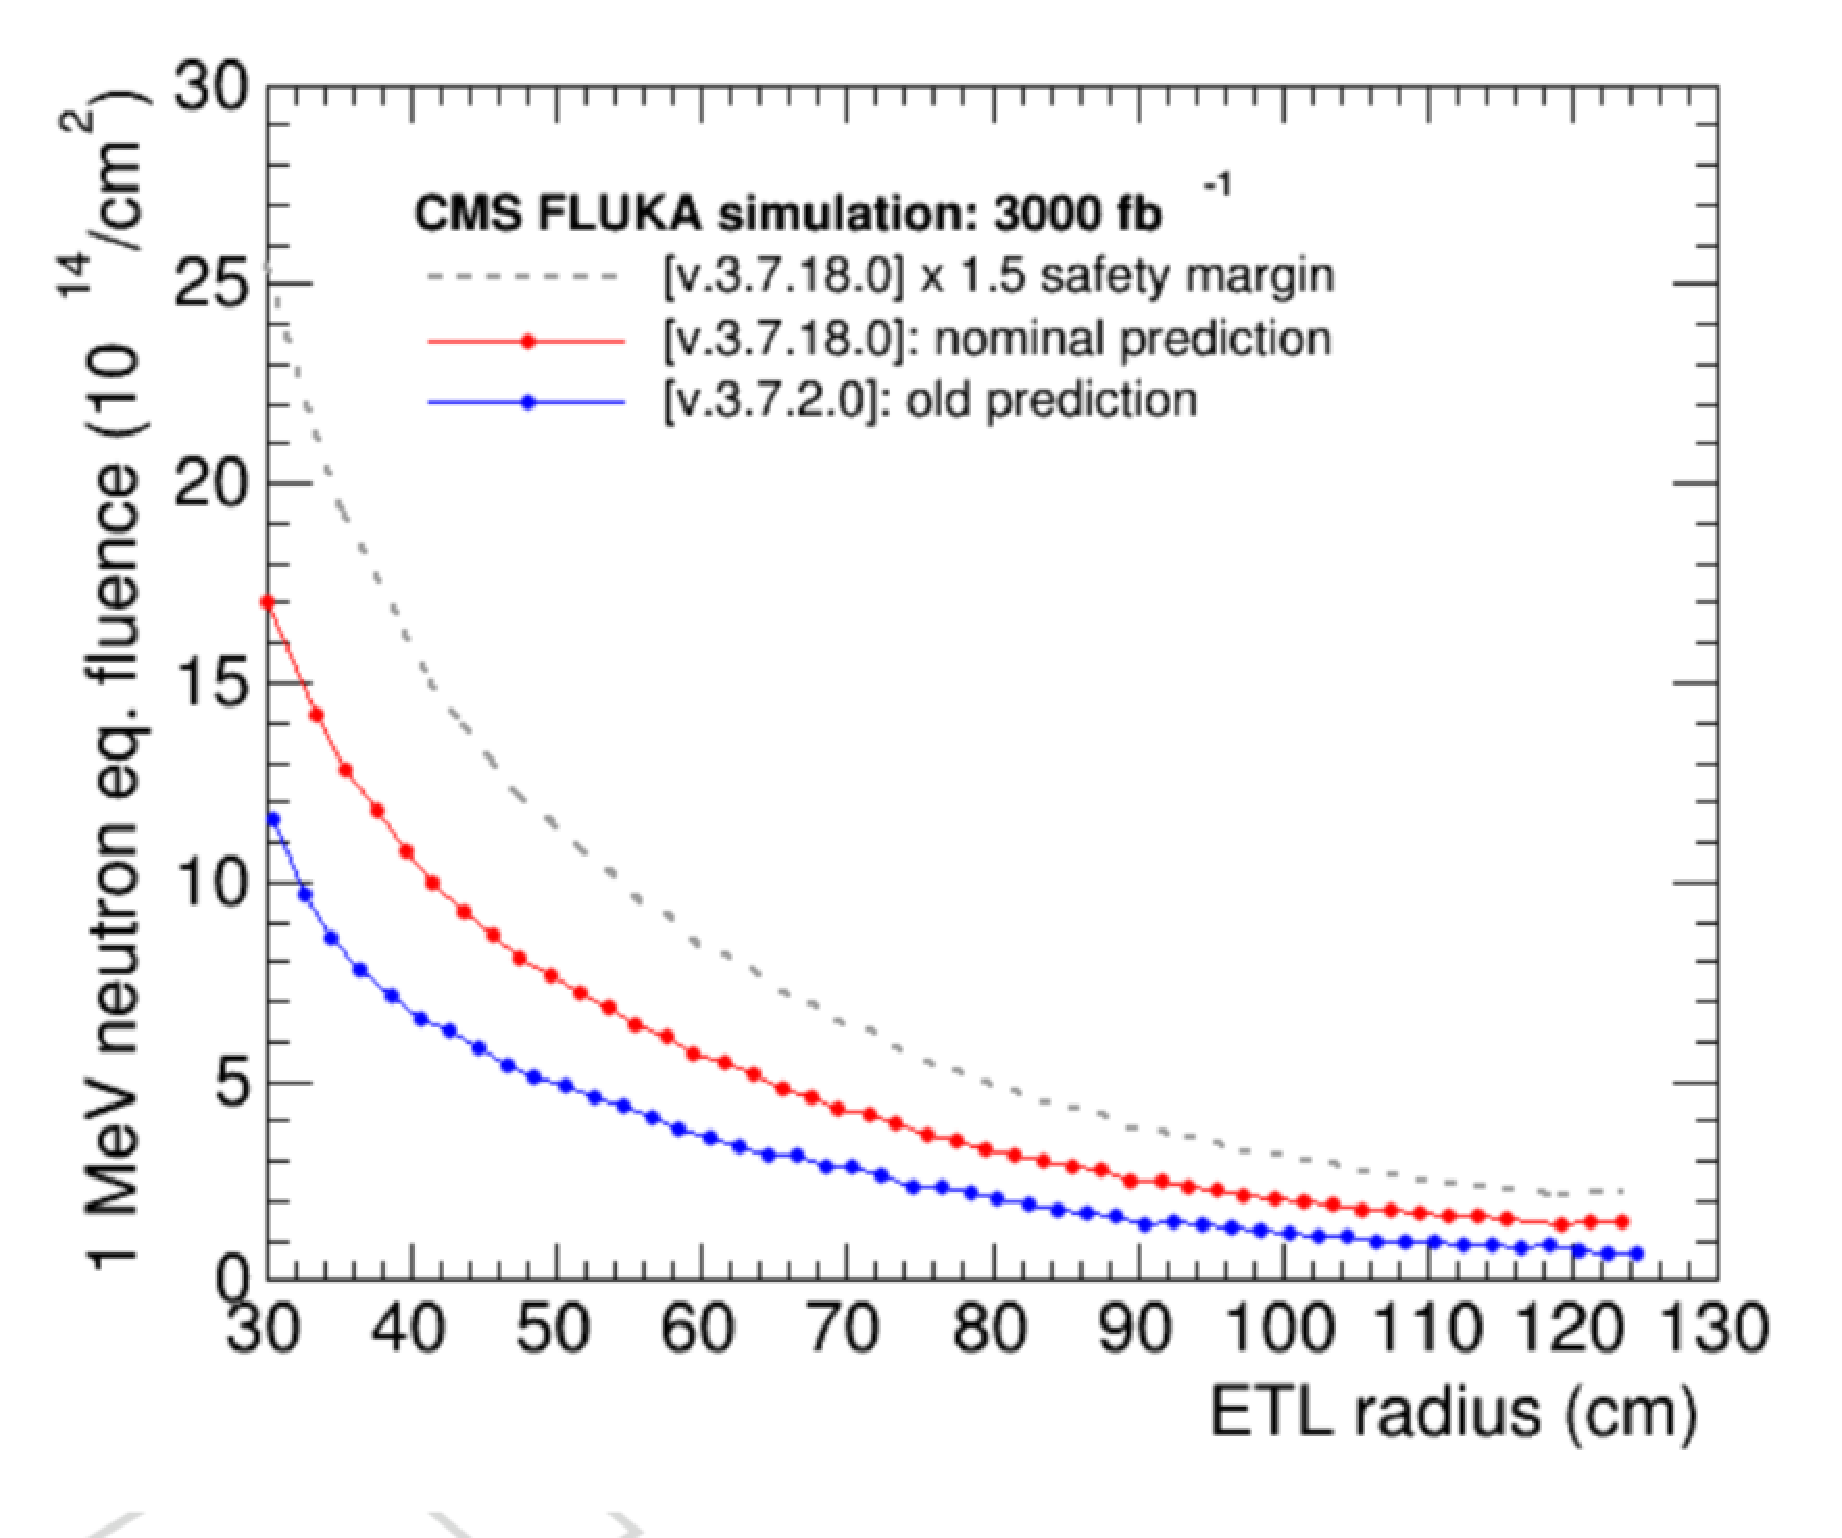
\includegraphics[width=\linewidth]{figures/image6.pdf}
\caption{
Fluence prediction in ETL for an integrated luminosity of 3000 fb$^{-1}$ from the FLUKA simulations.}
\label{fig:fluka}
\end{figure}

\section{Geometric Coverage}

We optimize the placement of modules and readout boards to achieve highest possible coverage of the ETL disk, without the need for half size modules.
The ETL disk is assumed to be limited by $r_{\mathrm{inner}}=315~\mathrm{mm}$ and $r_{\mathrm{outer}}=1185~\mathrm{mm}$, depicted by the red circles in Figure~\ref{fig:coverage_both}, corresponding to $1.659 \leq |\eta| \leq 2.950$ for an ETL position of $z=3~\mathrm{m}$.
Modules on the front and back face of each disk are arranged such that the area not covered by a sensor is minimized.
The two different arrangements are shown on the left and right of Figure~\ref{fig:coverage_both}.

In order to measure the coverage of the proposed module layout we use LGAD sensor dimensions of $22.0 \times 42.5~\mathrm{mm}$, and a full module of size $56.5 \times 43.1~\mathrm{mm}$.
A $0.5~\mathrm{mm}$ gap between each module is assumed, and the channel for the power board is taken to be $29.5~\mathrm{mm}$ wide.
Each side of the ETL detector is made of two disks (four faces) that are shifted by $2~\mathrm{mm}$ in $x$ and $y$ in order to also cover the inter-sensor gaps.

\begin{figure}[!h]
\centering
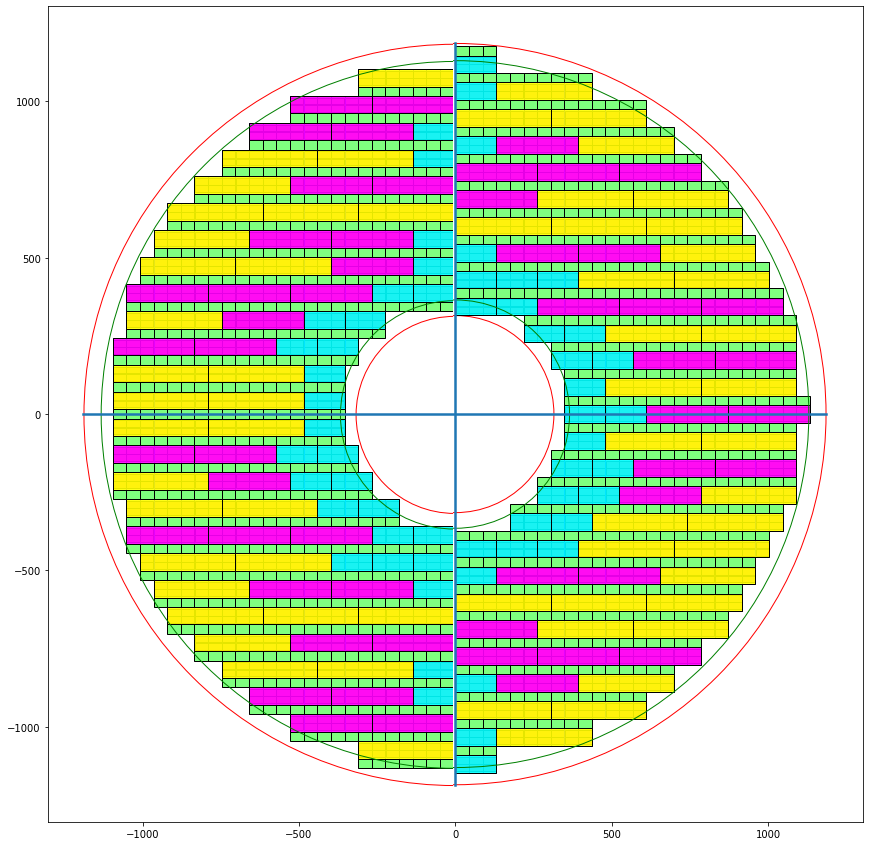
\includegraphics[width=0.60 \textwidth]{figures/coverage_both.png}
\caption{
Two half disks of the ETL detectors.
The red and green circles reflect the mechanical envelope of the ETL disk and the area between $1.7<|\eta|<2.8$, respectively.
Cyan, pink and yellow rectangles correspond to 3-, 6- and 7-module readout boards.
The green rectangles indicate the reserved space for the power boards and LV services.
}
\label{fig:coverage_both}
\end{figure}

Table~\ref{tab:coverage} shows the acceptance and geometric coverage of four different configurations of ETL modules on the disk.
The acceptance is measured by propagating muons produced at the center of CMS with $p_{T}>5~\mathrm{GeV}$ and a flat $\eta$ distribution through the CMS magnetic field to the ETL detector.
The different configurations correspond to the amount of space that is not covered by sensors at the outer edge of the disk in order to accomodate connectors (and potentially a mini-patch-panel for BV, LV and DSS).
The ``optimal'' configuration corresponds to the case where modules are placed up to the most outer edge of the disk, leaving no additional space for connectors.
In this case, 91\% of the area of the disk is covered by at least one sensor.
If 50, 65 or 85mm of space, measured along the x-axis from the modules, is kept free of modules, this geometric coverage reduces to 84--81\%.
However, due to the flat $\eta$ distribution that is used for the acceptance measurement with muons, the acceptance only reduces to 87--86\%.
For the region $1.70<|\eta|<2.80$ more than 97\% of muons intersect at least one sensor in any of the configurations.
%Approximately 96\% (70\%) of muons with $1.7<\eta<2.8$ and $p_{T}>25~\mathrm{GeV}$ produced at the center of CMS and propagated through the magnetic field have at least one (two) intersection with an ETL sensor.
An example of tracks and intersections with ETL sensors is shown in Fig.~\ref{fig:intersect}.
The majority of muons not producing any hit pass through uncovered areas at the edge of the ETL disks.
If the rapidity window is narrowed to $2.0<\eta<2.5$, more than 99\% of the muons intersect at least one of the sensors.

\begin{table}
  \caption{Acceptance for muons and geometric coverage of different configurations.}
  \label{tab:coverage}
  \begin{tabular}{c|cc|cc|cc}
    \multirow{2}{*}{Configuration} & \multicolumn{2}{c|}{$1.66<|\eta(\mu)|<2.95$} & \multicolumn{2}{c|}{$1.70<|\eta(\mu)|<2.80$} & \multicolumn{2}{c}{Geometric coverage} \\
                  & $\geq1$ hit & $\geq2$ hits  & $\geq1$ hit & $\geq2$ hits  & total & w.r.t. optimal \\ \hline
    optimal       & 0.91        & 0.79          & $>0.99$     & 0.91          & 0.91  & 1.00            \\
    50mm          & 0.87        & 0.75          & 0.99        & 0.91          & 0.84  & 0.924 \\
    65mm          & n/a         & n/a           & n/a         & n/a           & 0.83  & 0.915 \\
    85mm          & 0.86        & 0.75          & 0.97        & 0.90          & 0.81  & 0.894

  \end{tabular}
\end{table}

\begin{figure}[!h]
\centering
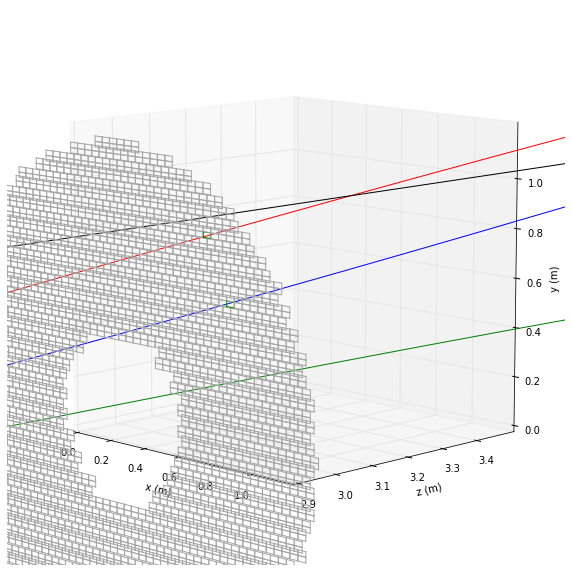
\includegraphics[width=0.70 \textwidth]{figures/intersect_3D.png}
\caption{
Tracks of three muons (red, blue, green) originating from the CMS interaction point, propagated through the CMS magnetic field.
Sensors of the first two faces of the ETL detector are shown.
Sensors that intersect the muon tracks are marked in green.
The green track passes the ETL detector without an intersection at the outer (low-$\eta$) edge of disk.
}
\label{fig:intersect}
\end{figure}

\section{Services}

LV distribution, Bias Voltage, Grounding, Cooling

At most five service hybrids are arranged in one row on the ETL disk, shown in Fig.~\ref{fig:coverage_both}.
Such a configuration is shown in Fig.~\ref{fig:services}.
LV cables can be routed on top of the PB, while the optical fibre bundles and BV cables will be routed on top of the RB.
MCT connectors for the fibres are located at the end of each row, and can be accompanied by small patch panels for LV, BV and DSS connection.

\begin{figure}[!h]
\centering
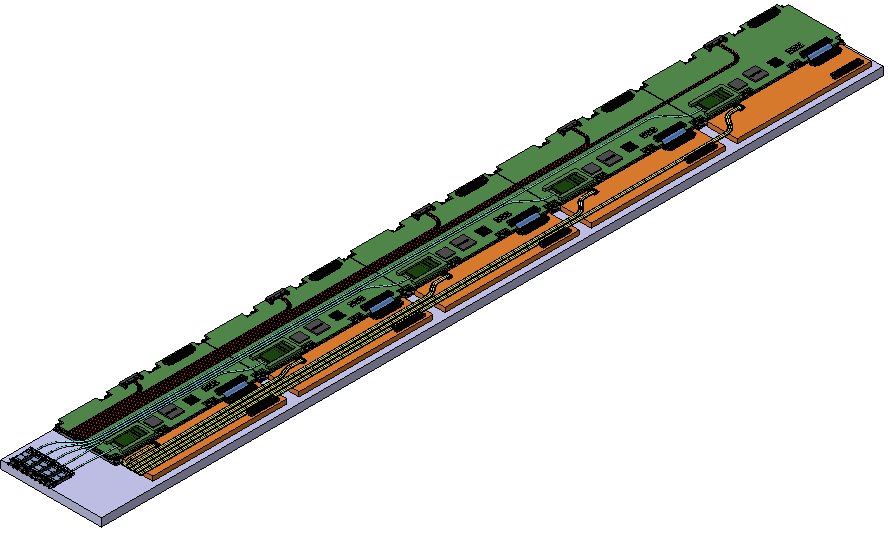
\includegraphics[width=0.90 \textwidth]{figures/services.png}
\caption{
Representation of the longest row of service hybrids, accomodating all necessary services (BV, LV, fibre bundles).
}
\label{fig:services}
\end{figure}

\section{Assembly and testing}

With the proposal at hand it is possible to assemble ``super-modules'' of the size of one readout board, which can then be tested and only subsequently get mounted on the ETL disk.
The assembly process would therefore be greatly simplified once the modules are assembled:
\begin{itemize}
  \item Connect modules one-by-one to the readout board
  \item If final assembly: Screw modules onto disk
  \item Connect BV cables to connectors on RB
  \item Connect RB to PB with flat cables.
\end{itemize}


\section{Summary}

The presented change of the ETL module and service hybrid design has several advantages over the TDR design:
\begin{itemize}
  \item Less space restrictions for RB and PB, especially vertically, giving more freedom in choice of components like capacitors
  \item Direct connection of RB to the module without flexi circuits, facilitating the assembly and testing processes
  \item PCB on modules allows for placement of components (e.g. bypass capacitors) close to the sensor and ETROCs
  \item No need for half sized modules
  \item Required stacking height of down to $7~\mathrm{mm}$ seems feasible
\end{itemize}

The following challenges have been identified:
\begin{itemize}
  \item Alignment and insertion force of board-to-board connectors
  \item Required space for MT connectors at the end of each row and associated loss of coverage at low $\eta$
\end{itemize}

\clearpage

\section{Bibliography}

\begin{itemize}
  \item [1]  C. Collaboration, "A MIP Timing Detector for the CMS Phase-2 Upgrade," CERN-LHCC-2019-003, 2019.
  \item [2]  S. Los, "Proposal for Readout Board on Top ETL SH Stack-up," 23 March 2020. [Online]. Available: https://indico.cern.ch/event/901444.
  \item [3]  A. Apresyan and W. Li, "ETL service hybrid prototyping plan," 2020. [Online]. Available: https://cms-docdb.cern.ch/cgi-bin/DocDB/ShowDocument?docid=14040.
  \item [4]  F. Faccio, "The bPOL12V DCDC converter for HL-LHC trackers: towards production readiness," in \emph{TWEPP}, Santiago de Compostela, 2019.
  \item [5]  J. Troska, A. Brandon-Bravo, S. Detraz, A. Kraxner, L. Olanterä, C. Scarcella, C. Sigaud, C. Soos and F. Vasey, "The VTRx+, an optical link module for data transmission at HL-LHC," in \emph{Topical Workshop on Electronics for Particle Physics}, Santa Cruz,, 2017.
  \item [6]  P. Moreira, "The lpGBT: a radiation tolerant ASIC for Data, Timing, Trigger and Control Applications in HL-LHC," in \emph{TWEPP}, Santiago de Compostela, 2019.
  \item [7]  A. Caratelli, S. Bonacini, K. Kloukinas, A. Marchioro, P. Moreira, R. De Oliveira and C. Paillard, "The GBT-SCA, a radiation tolerant ASIC for detector control and monitoring applications in HEP experiments," \emph{JINST,} vol. 10, no. 03, p. C03034, 2015.
  \item [8]  M. O. Sahin, "DAQ and clock -- status and schedule," in \emph{Timing Days}, CERN, 2020.
  \item [9]  K. DiPetrillo, "ETROC0 Tests with FEAST Based Switching Power Supply," ETL Meeting, 24 Nov 2019. [Online]. Available: https://indico.cern.ch/event/866436/.
  \item [10]  S. Los, "Power board prototyping plans," ETL Meeting, 29 April 2019. [Online]. Available: https://indico.cern.ch/event/816963.
  \item [11]  S. Lusin, "ETL Integration Issues," ETL meeting on sensors and modules, 6 Apr 2020. [Online]. Available: https://indico.cern.ch/event/906805/.
  \item [12]  CERN, "SAFETY INSTRUCTION IS23 - Criteria and Standard Test Methods for the Selection of Electric Cables and Wires with Respect to Fire Safety and Radiation Resistance," CERN, 2005. [Online]. Available:
    https://edms.cern.ch/ui/file/335745/4/E\_IS23.pdf.
  \item [13]  CERN, "Safety Instruction - The use of plastic and other Non-Metallic Materials at CERN with respect to Fire Safety and Radiation Resistance," CERN, 2005. [Online]. Available: https://edms.cern.ch/ui/file/335806/1.02/IS41\_E.pdf.
  \item [14]  P. Moreira, "lpGBT -- a User's Perspective," TWEPP, 17 Sep 2018. [Online]. Available:
  \item [15]  J. Olsen, "ETL DAQ and Fast Control: the view from ETROC/Front-end," ETL meeting (Front-End Electronics), 30 Mar 2020. [Online]. Available: https://indico.cern.ch/event/902740/.
\end{itemize}

\end{document}
